\providecommand{\StudySection}{\section}
\providecommand{\StudySubsection}{\subsection}

\StudySection{Choosing a strategy separately for each graph}
\label{sec:type-specialists}
A common predictor may miss differences in the work required by different graph structures. We therefore fit separate predictors for the seven graphs and enlarge the available seed strategies. The added choices can restrict seeding to maximal target sectors or reduce numerator seeding in lower sectors through Kira's truncation option~\cite{Kira3}. Each method first enforces a valid positive-index bound for its declared sectors, and the final basis check and fallback remain in place.

For each graph, ten candidate models predict the complete-time ratios of nine strategies from nine target and family features. The candidates include regression trees, a bagged ensemble of trees, regularized linear models, and nearest-neighbour models. Their cost labels include unsuccessful attempts and retries. The data contain 36 training batches, 18 validation batches, and 36 reserved test batches at new rational parameter values, with $d$ symbolic throughout. Targets include propagator powers up to three, lower sectors, and auxiliary numerator indices $-2$. Appendix~\ref{app:type-specialists} gives the exact input definitions and selection procedure.

Training and validation contain 2,798.5 seconds of measured reductions, while fitting all seventy candidates takes 0.86 seconds. These offline costs exclude reference construction, development, and replaced measurements and are not included in application time. Validation enables a new predictor only if it saves at least five percent against the fastest available control. The controls are native choices, a deterministic sector-and-truncation rule, and a fixed strategy for each graph selected from training; the fixed strategy may itself use the older equation filter. This requirement activates predictors for three graphs and retains a control for the others. Unknown graphs and features outside the training range use native choices.

Five repetitions of four methods give 720 test calculations, all of which pass exact coefficient checks. With equal weight for each graph, the selected method has ratio $0.9368$ to native choices, with descriptive interval $[0.8867,0.9878]$, corresponding to 6.3\% less time. Its ratio to a fixed strategy for each graph is $0.9441$ with interval $[0.8992,0.9863]$. This second comparison isolates the benefit of selecting a strategy from the targets beyond choosing one setting for the whole graph.

Table~\ref{tab:type-specialists} shows lower time for five of the seven groups. The enabled trees save 14.2\% for the planar box, 12.4\% for the ladder, and 13.8\% for the nonplanar box. The vacuum and box with external virtuality take 3.7\% and 0.8\% more time, respectively, while retaining control strategies throughout. In particular, the vacuum uses native settings, so its difference includes the extra selection overhead and execution variation. Across 180 timed trials, the selected method needs no retries and native choices require 40; these costs are included in the ratios.

\begin{table}[!htbp]
\centering\small
\caption{Reduction time with a separate strategy for each graph. Times are geometric means of batch medians in seconds, and the ratio divides selected time by native time. The strategy column identifies the enabled model or retained control.}
\label{tab:type-specialists}
\begin{tabular}{@{}llrrr@{}}\toprule
Graph & Strategy & Native & Selected & Ratio\\\midrule
Sunrise & Stronger truncation & 0.825 & 0.811 & 0.983\\
Planar box & Depth-two tree & 3.410 & 2.925 & 0.858\\
Vacuum & Native & 1.033 & 1.072 & 1.037\\
Ladder & Depth-one tree & 5.144 & 4.506 & 0.876\\
Nonplanar box & Depth-two tree & 6.234 & 5.376 & 0.862\\
Pentagon & Target sectors & 1.040 & 0.989 & 0.951\\
Virtuality box & Sectors and truncation & 0.808 & 0.815 & 1.008\\
\bottomrule\end{tabular}
\end{table}

\begin{figure}[!htbp]
\centering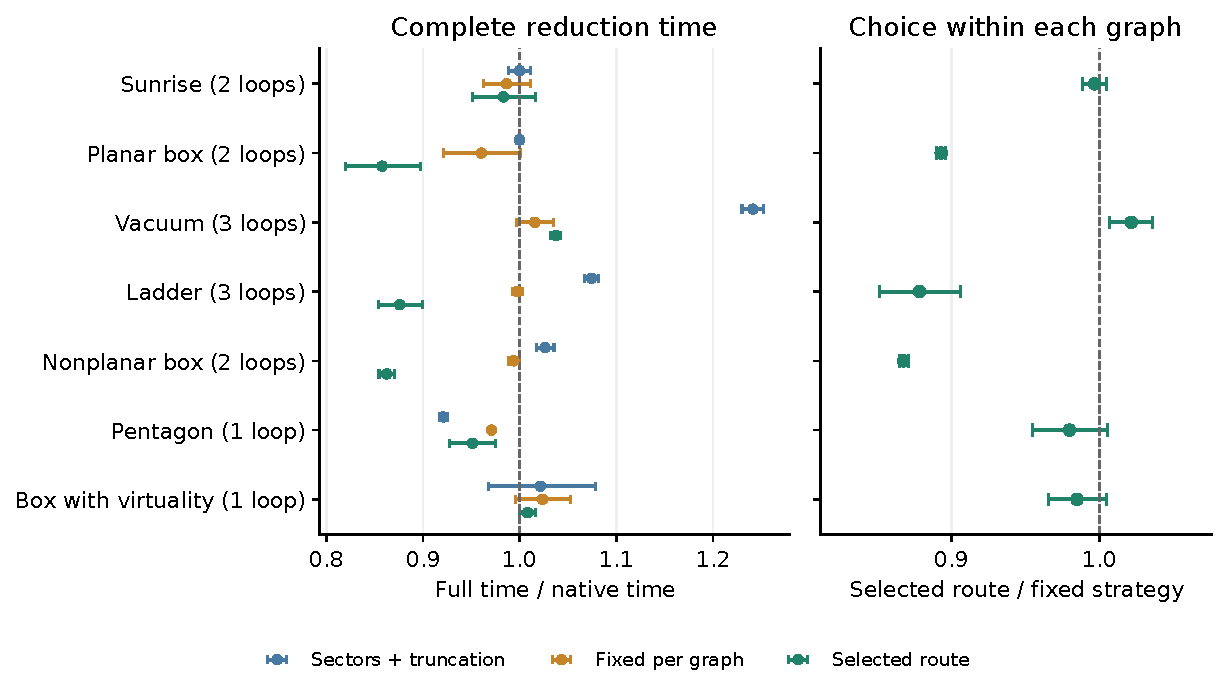
\includegraphics[width=\linewidth]{paper_figures/type_specialists.pdf}
\caption{The effect of choosing a separate policy for each graph.
Left: complete-time ratios to native choices. Right: the selected method
relative to one fixed strategy per graph. Bars show the range across two
reserved parameter profiles; they are not significance intervals.
Both panels retain the equal-time reference.}
\label{fig:type-specialists}
\end{figure}

\FloatBarrier

The timed trials check 14,040 coefficient entries. A further 36 applications supplied only with the master basis and seven additional application checks verify 945 coefficients independently. These checks establish correct completion for the measured inputs. The graph structures and target patterns are known during training, and each graph has only two training parameter profiles. The reserved profiles therefore test new kinematic values within these inputs, leaving new target structures and general scattering beyond three loops for further study.
